
To compare SN rates in clusters of different ages, rate measurements
must be normalized by stellar mass rather than stellar luminosity
because luminosity changes as stars age. To convert our luminosity
measurements to mass measurements we use a mass-to-light ($M/L$) ratio
based on a stellar evolution model. There are several available models
in the literature. The choice of stellar tracks, metallicity, star
formation history, and in particular the assumed IMF, will all affect
the derived $M/L$ ratio to some extent. For the purpose of measuring
the change in rate with redshift, it is important to use a
\emph{consistent} model and assumptions for determining the $M/L$
ratio for all rate measurements. That is, we are most concerned that
the model accurately captures the evolution of stellar luminosity over
the redshift range of interest ($0<z<1.46$), and less concerned about
the overall normalization of the $M/L$ ratio. To that end, for our
main result we will use a model and assumptions that match as closely
as possible those used for the $M/L$ ratio in low-redshift cluster
rate measurements. As we also give results normalized by luminosity,
those wishing to use a different $M/L$ ratio can easily do
so. Finally, note that the \emph{initial} stellar mass formed is the
quantity of interest for normalizing rate measurements. However, as
most rate measurements and $M/L$ ratios have been reported in terms of
current mass, we give our results in these units and simply note the
difference between current and initial mass for the purpose of
comparing rate measurements. Thus, in the following paragraphs $M$
refers to current stellar mass.

\subsubsection{$M/L$ ratio in low-redshift cluster rate measurements}

The lower-redshift cluster rate studies
of \citet{sharon07a}, \citet{sharon10a}, and by
extension, \citet{dilday10a} have used the relations between $M/L$
ratio and galaxy color derived by \citet[][hereafter Bell03]{bell03a}.
For example, \citet{sharon07a} use the relation $\log_{10} (M/L_z) =
-0.052 +0.923(r-i)$ and \citet{sharon10a} use $\log_{10} (M/L_g) =
-0.499 +1.519(g-r)$, where $M$, $L_z$ and $L_g$ are in solar units.
In order to use a consistent model, it is important to recognize how
these relations were derived.  Bell03 fit a grid of {\sc
p{\'e}gase2} \citep{fioc97a} synthetic galaxy spectral energy
distributions (SEDs) to actual $ugrizK$ photometry of low-redshift
galaxies. The grid covers a range of metallicities and star formation
histories. The star formation histories have exponentially-decreasing
or -increasing star formation rates, and assume that star formation
commenced at $z=4$. For each galaxy, the $M/L$ ratio is that of the
best-fit synthetic galaxy SED, consistently evolved to $z=0$.  Bell03
use a ``diet'' \citet{salpeter55a}
IMF \citep[following][]{bell01a}. This IMF is defined as having the
same colors and luminosity as a Salpeter IMF, but with a total mass
30\% lower. The difference in mass is attributed to a smaller number
of faint low-mass stars relative to a Salpeter IMF. These stars do
not contribute significantly to the luminosity of the Salpeter
IMF. The diet Salpeter IMF results in $M/L$ ratios 30\% lower at a
given color than a normal Salpeter IMF. Note that because Bell03
simply take the $M/L$ ratio from the best-fit synthetic SED of each
galaxy, the Bell03 relations will generally fall within the grid of
$M/L$ versus color covered by the synthetic galaxy SEDs.

%%%%%%%%%%%%%%%%%%%%%%%%%%%%%%%%%%%%%%%%%%%%%
% PLOT: MASS-TO-LIGHT RATIOS                %
%%%%%%%%%%%%%%%%%%%%%%%%%%%%%%%%%%%%%%%%%%%%%
\begin{figure}
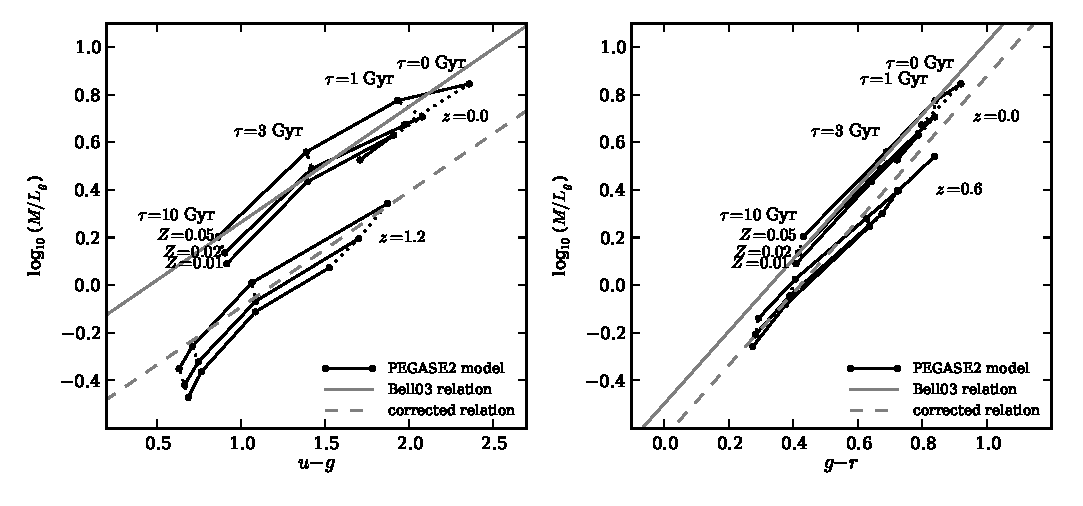
\includegraphics[width=\textwidth]{figures/clrate/mlratio.eps}
\caption[Evolution of $M/L$ ratio versus color with redshift]
{Evolution of $M/L$ ratio versus color with redshift. 
\emph{Left panel:} $M/L$ ratio as a function of $u-g$ color 
at $z=0$ and at $z=1.2$ (typical redshift in this study). The grid of
points show {\sc p{\'e}gase2} models with exponentially-decreasing
star formation rates with e-folding times $\tau$ and metallicities
$Z$. For each model, star formation begins at $z=4$. Models with
constant metallicity are connected by solid black lines and models
with identical star formation histories are connected by dotted
lines. For example, models with $\tau = 0$, corresponding to a simple
stellar population, are the rightmost points (corresponding to
$Z=0.01$, $0.02$, $0.05$) connected by dotted lines. As the models are
evolved back in time from an observed redshift of $z=0$ to an observed
redshift of $z=1.2$, the $M/L$ ratio decreases and moves away
from the Bell03 relation (solid grey line). The dashed
grey line shows the relation used in this study for $z=1.2$. At
$z=1.2$ the offset from the Bell03 relation is $-0.36$~dex, or a
factor of 0.43. \emph{Right panel:} Same as left panel, but for $g-r$
color and for an observed redshift of $z=0.6$, the typical redshift in
the rate study of \citet{sharon10a}. The offset here is only
$-0.14$~dex, or a factor of 0.72.
\label{fig:mlratio}}
\end{figure}

\subsubsection{$M/L$ ratio at $0.9<z<1.46$}

Ideally, for consistency with \citet{sharon07a}, \citet{sharon10a}
and \citet{dilday10a}, we would simply use the Bell03 relation for
$u-g$ color, which most closely matches our observed color: $\log_{10}
(M/L_g) = -0.221 +0.485(u-g)$. However, the Bell03
relations are based on $ugrizK$ photometry of low-redshift galaxies,
corrected for evolution to $z=0$. As such, they are specific to $z=0$
and not directly applicable at high redshift. A stellar population
passively evolving from age a few~Gyr (at $z \sim 1$) to $> 10$~Gyr
(at $z=0$) will dim significantly while only growing slightly redder
(see, e.g. BC03), in a manner that does not follow the Bell03
relations.  To estimate the effect of evolution from their $z=0$
relation to higher redshift, we make a similar grid of {\sc
p{\'e}gase2}-generated SEDs with the same formation redshift,
metallicities, IMF, and star formation histories. As expected, when
evaluated at $z=0$, the $M/L$ ratios of this grid are consistent with
the Bell03 relation (Fig.~\ref{fig:mlratio}, left panel, upper grid of
black points). Evaluating the SEDs at higher redshifts, we find that
the $M/L$ ratios are well fit by a relation with the same slope, but
smaller normalization. For example, at $z=1.2$, the best-fit offset
from the $z=0$ relation is $-0.36$~dex (Fig.~\ref{fig:mlratio}, left
panel, dashed line). At the extremes of the redshift range of
interest, the best fit offset is $-0.26$~dex ($z=0.9$) and $-0.44$~dex
($z=1.46$). We therefore use a $M/L$ ratio of
\begin{equation} \label{eq:mlratio}
\log_{10} (M/L_g) = \left\{ \begin{array}{ll}
-0.48+0.485(u-g), & z=0.9 \\
-0.66+0.485(u-g), & z=1.46
\end{array} \right.
\end{equation}
and linearly interpolate for intermediate redshifts. Another way to
view Equation~(\ref{eq:mlratio}) is that, independently of the
relation at $z=0$, we have fit a linear relation to the {\sc
p{\'e}gase2} SEDs at the redshift of each cluster, assuming a slope
consistent with Bell03.

%This is motivated by the fact
%that the models seem to indicate a similar slope, and also by the fact
%that small changes in the slope will not make a big difference in the
%result. This is because most of the cluster light is in galaxies
%confined to a narrow range in color ($1.3 < u-g < 1.7$).


%%%%%%%%%%%%%%%%%%%%%%%%%%%%%%%%%%%%%%%%%%%%%
% PLOT: COLOR HISTOGRAM                     %
%%%%%%%%%%%%%%%%%%%%%%%%%%%%%%%%%%%%%%%%%%%%%
\begin{SCfigure}[0.7][tb]
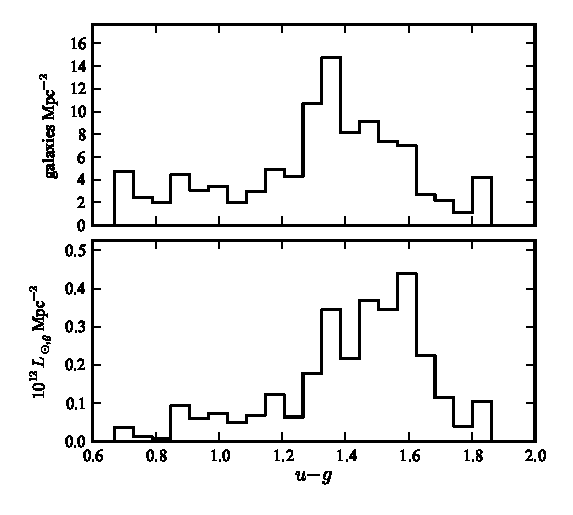
\includegraphics[width=0.65\textwidth]{figures/clrate/colorhist.eps}
\caption[Distribution of cluster galaxy rest-frame colors]
{Stacked distribution of galaxy rest-frame colors for all 
25 clusters. The background (based on the GOODS fields) has been
statistically subtracted. Only galaxies within $0.5$~Mpc of cluster
centers have been included in order to limit variance from the
background. The \emph{top panel} shows galaxy density in each color bin,
while in the \emph{bottom panel} the distribution is weighted by galaxy
luminosity.
\label{fig:colorhist}}
\end{SCfigure}

Using Equation (\ref{eq:mlratio}) we calculate mass on a
galaxy-by-galaxy basis: we $K$-correct the observed $i_{775}$ and
$z_{850}$ magnitude to rest-frame SDSS $u$ and $g$ magnitudes using
the method discussed in \S\ref{sec:lum_kcorr}, and obtain the $M/L$
ratio from the $u-g$ color. In all, 66\% of the clusters'
luminosity is from galaxies with color in the range $1.3 < u-g < 1.7$,
27\% of the luminosity is distributed roughly equally between galaxies
in the range $0.6 < u-g < 1.3$, and the remainder is in redder
galaxies with $u-g > 1.7$ (Fig.~\ref{fig:colorhist}). Thus, while there is a clear presence of
bluer cluster galaxies, the majority of the clusters luminosity is
confined to a narrow range in color. This narrow color range means
that changes in the assumed slope of Equation (\ref{eq:mlratio}) will
not have a large effect on the resulting total mass.

The cumulative $M/L$ ratio (the ratio of the total mass of all 25
clusters to the total luminosity of all 25 clusters) is $M/L_g = 1.25$
(see Table~\ref{tab:clrates}, ``denom''). For red-sequence galaxies
only, the ratio is higher ($M/L_g = 1.38$) due to the exclusion of
bluer galaxies with a lower inferred $M/L$ ratio.

\subsubsection{$M/L$ ratio uncertainty}

As noted above, we are primarily concerned with the accuracy of the
evolution in the stellar mass and luminosity over the range
$0<z<1.46$, rather than the accuracy of the absolute $M/L$ ratio.  As
a cross-check of the $M/L$ ratio evolution, we have compared the above
results (using {\sc p{\'e}gase2}) to the results obtained with the
BC03 SEDs. We use the standard Padova 1994 evolution and the same star
formation histories as above. In terms of evolution offset from $z=0$
to $z \sim 1.2$, we find results consistent within 0.03~dex.

This consistent evolution in BC03 and {\sc p{\'e}gase2} is
encouraging. However, to be much more conservative in our estimate of
the uncertainty in the $M/L$ ratio evolution, we take the scatter of
the models around the best-fit line as our uncertainty. In
Figure~\ref{fig:mlratio}, in the color range of interest, the scatter
is approximately $\pm 0.08$~dex (20\%) at both low and high
redshift. We use this as the systematic uncertainty in the $M/L$ ratio
for the purpose of comparing SN rates at low and high redshift
in \S\ref{conclusionsdtd} and \S\ref{conclusionssys}. The uncertainty
in the absolute $M/L$ ratio is much greater, due mainly to the
uncertainty in the true IMF.

%If, instead of using a
%color-dependent $M/L$ ratio, we had used a constant $M/L$ ratio of
%1.38 (derived from redder, older galaxies) we would make an error in
%the total mass of order $\sim 10\%$. Thus, while it is important to
%account for a lower $M/L$ ratio in bluer galaxies, small changes in
%the slope will only incur errors of much less than 10\%.

%For reference, the $M/L$ ratio of a BC03 starburst
%with $Z=0.02$ and age 3~Gyr (the age of a cluster at $z \approx 1.18$
%with $z_f = 3$) is $M_\odot/L_{g,\odot} = 1.42$.


%%%%%%%%%%%%%%%%%%%%%%%%%%%%%%%%%%%%%%%%%%%%%%%%%%%%%%%%%%%%%%%%%%%%%
%\NOTE{why z band is OK}
%The observed $z_{850}$ band corresponds to approximately rest-frame
%$B$-band for the most of the clusters. In general, $B$-band luminosity
%is not a good tracer of stellar mass, as it is sensitive to small
%amounts of young stars \citep[see, e.g.][]{mannucci05a}. However, the
%majority of the cluster light comes from red-sequence galaxies with
%little or no recent star formation.  For these galaxies, $B$-band
%light is not heavily affected by young stars and provides a reasonable
%stellar mass estimate. Still, to account for a reduced $M/L$
%ratio in the bluer cluster galaxies, we use a color-dependent
%$M/L$ ratio and the observed $i_{775}-z_{850}$ galaxy color to
%obtain a $M/L$ ratio on a galaxy-by-galaxy basis.
%
%%%%%%%%%%%%%%%%%%%%%%%%%%%%%%%%%%%%%%%%%%%%%%%%%%%%%%%%%%%%%%%%%%

%To do this we make a grid of synthetic galaxy spectral energy
%distributions (SEDs) using {\sc p{\'e}gase} \citep{fioc97a} and
%compare $M_\odot/L_{g,\odot}$ versus $u-g$ at different
%redshifts. Each SED has an exponentially-declining star formation
%rate, with time constants ranging from $\tau = 0$ (instantaneous
%burst) to $\tau = \infty$ (continuous star formation). Metallicities
%range from $Z = 0.0004$ to $Z=0.02$, and the formation redshift (onset
%of star formation) ranges from $z_f=3$ to $z_f=6$, with the
%corresponding age calculated accordingly. (At redshifts $z=0$,
%$z=0.9$, and $z=1.45$, the corresponding age range is 11.3 to
%12.5~Gyr, 4.0 to 5.2~Gyr, and 2.2 to 3.4~Gyr, respectively). For each
%SED, we calculate the $u-g$ color and $M/L_{g,\odot}$, using the
%tabulated values of remaining stellar mass. We find that at both $z=0$
%and $z=0.9$, the older and redder SEDs (with $\tau \lesssim 2$~Gyr)
%follow a slope in $M_\odot/L_{g,\odot}$ versus $u-g$ consistent with
%the Bell03 relations, both in normalization and slope. However, at
%$z=0.9$, the best-fit offset is $0.26$~dex smaller than at $z=0$. At
%$z=1.45$, the offset is $0.44$~dex smaller than at $z=0$. We therefore
%use a mass-to-light ratio of $\log_{10} (M_\odot/L_{g,\odot}) = -0.48
%+0.485(u-g)$ at $z=0.9$ and $\log_{10} (M_\odot/L_{g,\odot}) = -0.66
%+0.485(u-g)$ at $z=1.45$, linearly interpolating for intermediate
%redshifts.
